\documentclass[11pt,a4paper]{article}

\usepackage[utf8]{inputenc}
\usepackage[T1]{fontenc}
\usepackage{lmodern}
\usepackage[margin=2.45cm]{geometry}
\usepackage{amsmath,amssymb,amsfonts}
\usepackage{booktabs}
\usepackage{array}
\usepackage{graphicx}
\usepackage{xcolor}
\usepackage{hyperref}
\usepackage{enumitem}
\usepackage{longtable}

\hypersetup{
  colorlinks=true,
  linkcolor=blue!50!black,
  citecolor=blue!50!black,
  urlcolor=blue!50!black
}

\setlist[itemize]{topsep=2pt,itemsep=2pt,parsep=0pt}
\setlist[enumerate]{topsep=2pt,itemsep=2pt,parsep=0pt}
\renewcommand{\arraystretch}{1.16}

\newcommand{\TACM}{\mathrm{TACM}}
\newcommand{\Var}{\mathrm{Var}}
\newcommand{\Bin}{\mathrm{Binomial}}
\newcommand{\Unif}{\mathrm{Uniform}}
\newcommand{\Qtail}{Q_{\mathrm{tail}}}
\newcommand{\KS}{\mathrm{KS}}
\newcommand{\Neff}{N_{\mathrm{eff}}}

\title{\textbf{TACM / PRNG Structural Diagnostics}\\
\large Empirical Measures, Seed-Conditioned Variance, Null Calibration and Reproducibility Boundaries}
\author{Pascal Montmory}
\date{May 2026}

\begin{document}
\maketitle

\noindent\textbf{Scope and evidentiary policy.} This manuscript presents the TACM / PRNG structural diagnostics framework as a self-contained contribution. It defines the diagnostic objects, states the non-claims, develops empirical-measure and seed-conditioned Monte Carlo diagnostics, introduces a null-calibrated variance test, and reports a reproducible CPU-only baseline. Claims are explicitly labelled as definitions, reproducible evidence, reported evidence requiring archival raw logs for independent verification, or stated limitations.

\begin{abstract}
This manuscript introduces TACM, a structural diagnostic framework for pseudo-random number generators under finite Monte Carlo workloads. TACM is formulated around empirical measures of PRNG output, seed-conditioned replicated Monte Carlo estimators, null-calibrated variance diagnostics, ECDF interpretation and exact rare-event calibration.

The central position is that TACM does not replace established PRNG batteries such as TestU01 or BigCrush. Instead, it adds a Monte Carlo workload-facing layer: it measures how seed-conditioned PRNG streams affect replicated Monte Carlo estimators. The core calibrated diagnostic is
\[
Z_s(f)=F_{\chi^2_{R-1}}
\left(
\frac{(R-1)V_s(f)}{\sigma_f^2/N}
\right),
\]
where $V_s(f)$ is the empirical variance of replicated Monte Carlo estimates under seed $s$.

The verified CPU-only baseline in this document tests four public NumPy bit generators, four integrands, $S=1000$ seeds, $R=8$ replicates and $N=50\,000$ draws per replicate. It shows that large raw max/min variance ratios occur naturally, but after null calibration the tested public PRNGs do not show strong tail-pathological behaviour on these simple workloads. Several generator/integrand pairs show mild calibration drift; none clearly survives a strict Bonferroni correction at $m=16$, and exact binomial rare-event PIT checks are compatible for all four public generators.

Reported TestU01 / BigCrush results and cross-backend Montmory\_CTACM observations are included as reported evidence requiring archival raw logs and stream hashes for independent verification. They are not treated as independently reproducible evidence in the present manuscript.
\end{abstract}

\clearpage
\tableofcontents
\clearpage

\section{Scientific Positioning}

\subsection{What TACM is}

TACM is a structural diagnostic framework for PRNG behaviour under finite Monte Carlo workloads. It studies objects of the form
\[
\Phi(G,p,s,N),
\]
where $G$ is a deterministic generator, $p$ a parameter setting, $s$ a seed, $N$ a finite horizon, and $\Phi$ a declared observable such as a Monte Carlo estimator, empirical transition matrix, empirical measure or cross-backend replay hash.

The practical question is:
\[
\boxed{
\text{How much does the seed affect Monte Carlo outputs under a declared workload?}
}
\]

\subsection{What TACM is not}

TACM is not:
\begin{itemize}
  \item a replacement for TestU01, PractRand, BigCrush or other stream-level batteries;
  \item a proof of randomness;
  \item a proof of cryptographic security;
  \item a theorem about all seeds, all horizons or all workloads unless such a theorem is explicitly provided;
  \item a validation of any proprietary generator merely from summary tables.
\end{itemize}

The strict non-claim is:
\[
\boxed{
\text{Empirical randomness tests are evidence, not proof.}
}
\]

\subsection{What is new in the consolidated version}

Compared with the initial v1.0 document, this consolidated version adds:
\begin{itemize}
  \item the empirical-measure formulation of PRNG output;
  \item a careful separation between raw ratios and calibrated evidence;
  \item the null-calibrated diagnostic $Z_s(f)$;
  \item ECDF and tail-rate interpretation;
  \item exact binomial rare-event PIT checks;
  \item a reproducible CPU-only public-generator baseline with $S=1000$ seeds;
  \item explicit evidence-status labels for all non-reproducible reported results.
\end{itemize}

\section{Evidentiary Status of Claims}

\small
\begin{longtable}{
>{\raggedright\arraybackslash}p{0.25\textwidth}
>{\raggedright\arraybackslash}p{0.35\textwidth}
>{\raggedright\arraybackslash}p{0.30\textwidth}}
\caption{Evidentiary status of claims used in this manuscript.}\\
\toprule
Item & Content & Status \\
\midrule
\endfirsthead
\toprule
Item & Content & Status \\
\midrule
\endhead
Definitions & PRNG tuple, seed model, observables, empirical measures, replicated variance & Verified definitions. \\
Formulae & $\chi^2$, projected transition diagnostics, $V_s(f)$, $\rho_f$, $Z_s(f)$, $\Qtail$ & Mathematical definitions / diagnostic formulas. \\
Public CPU baseline & MT19937, PCG64, Philox, SFC64; $S=1000$, $R=8$, $N=50\,000$ & Reproducible local evidence; CSV, scripts and figures available. \\
Exact binomial rare-event PIT & Randomized binomial PIT for $1_{\{u>0.99\}}$ reconstructed from estimates & Reproducible local evidence; summary CSV generated. \\
Montmory\_CTACM BigCrush & Reported $160/160$ on x86, Metal and CUDA & Reported evidence; raw logs required for independent verification. \\
Montmory\_CTACM cross-backend replay & Reported bit-exact CPU/Metal/CUDA single-lane equality & Reported evidence; stream hashes required for independent verification. \\
Earlier inter-seed dispersion table & $N=10^6$, $R=8$, 100 seeds, multiple PRNGs & Reported evidence; raw tables required for independent verification. \\
Power tests & injected marginal bias, temporal correlation, rare-event deletion & Future work unless commands and outputs are added. \\
Security claims & unpredictability, cryptographic strength, adversarial resistance & Not claimed. \\
\bottomrule
\end{longtable}
\normalsize

\section{PRNG Model and Seed Model}

\subsection{Generator model}

A deterministic PRNG instance is represented as
\[
G=(S,P,A,T,O,U),
\]
where $S$ is the state space, $P$ the parameter space, $A$ the output alphabet, $T_p:S\to S$ the state transition, $O_p:S\to A$ the output map, and $U:A\to[0,1)$ the map from output words to Monte Carlo uniforms.

Given initial seed $s_0$ and parameter value $p$,
\[
s_{t+1}=T_p(s_t),
\qquad
x_t=O_p(s_t),
\qquad
u_t=U(x_t).
\]
For a finite horizon $n$, write
\[
X_n(p,s)=(x_0,\ldots,x_{n-1}),
\qquad
U_n(p,s)=(u_0,\ldots,u_{n-1}).
\]
All empirical claims in this document are finite-window claims unless a theorem explicitly states otherwise.

\subsection{Seed model}

A seed model is a probability law or finite test set over a declared seed domain, together with an initialization map
\[
\mathrm{Init}_p:\mathrm{Seed}\to S.
\]
The caller seed and the effective internal state need not be identical.

Seed perturbation rules can be expressed as
\[
N_\delta:\mathrm{Seed}\to\mathcal P(\mathrm{Seed}).
\]
Examples include one-bit flips, bounded Hamming perturbations and modular additive neighbourhoods:
\[
N_{\mathrm{1bit}}(s)=\{s\oplus 2^j:0\leq j<w\},
\]
\[
N_{\mathrm{add},k}(s)=\{(s+r)\bmod 2^w:-k\leq r\leq k\}.
\]

\subsection{Observables}

An observable is a declared function on a finite word or uniform window:
\[
\Phi:A^n\to\mathbb R^d,
\qquad
\Phi:[0,1)^n\to\mathbb R^d.
\]
Examples include bit frequencies, transition matrices, TestU01 scores, empirical measures, backend hashes and Monte Carlo estimates.

A seed-impact claim must specify:
\begin{itemize}
  \item generator and parameters;
  \item seed model;
  \item perturbation rule or seed set;
  \item output horizon;
  \item observable;
  \item proof, exact enumeration, or reproducible empirical protocol.
\end{itemize}

\section{Empirical Measures of PRNG Output}

For a seed $s$, backend $b$ and horizon $N$, the marginal empirical measure is
\[
\mu^{(1)}_{s,b,N}
=
\frac1N\sum_{t=1}^{N}\delta_{u_{s,b,t}}.
\]
The ideal marginal target is the Lebesgue measure $\lambda$ on $[0,1)$.

Temporal dependence is represented by block empirical measures:
\[
\mu^{(k)}_{s,b,N}
=
\frac1{N-k+1}
\sum_{t=1}^{N-k+1}
\delta_{(u_{s,b,t},\ldots,u_{s,b,t+k-1})},
\qquad k\geq2.
\]
The ideal target is $\lambda^{\otimes k}$.

The structural principle is:
\[
\boxed{
\parbox{0.86\textwidth}{\centering
A useful PRNG for Monte Carlo should produce empirical measures stable across seeds, backends and workloads.}
}
\]

\section{Classical and Projected Diagnostics}

\subsection{Marginal coverage}

Partition $[0,1)$ into $m$ bins $I_1,\ldots,I_m$. For seed $s$:
\[
O_i(s)=\#\{t:u_{s,t}\in I_i\},
\qquad
E_i=\frac Nm.
\]
The $\chi^2$ statistic is
\[
\chi^2_s=\sum_{i=1}^{m}\frac{(O_i(s)-E_i)^2}{E_i},
\qquad
\chi^2_{\mathrm{norm}}(s)=\frac{\chi^2_s}{m-1}.
\]
This measures marginal bin coverage, not temporal mixing.

\subsection{Projected transition diagnostics}

Define a quantizer
\[
Q_q:[0,1)\to\{1,\ldots,q\},
\qquad
b_t=Q_q(u_t).
\]
The row-stochastic empirical transition matrix is
\[
P_s(i,j)=
\frac{\#\{t:b_t=i,\ b_{t+1}=j\}}
{\#\{t:b_t=i\}}.
\]
This is a finite Markov projection of the observed stream, not the internal dynamics of the PRNG.

If
\[
1=\lambda_1,\lambda_2,\ldots,\lambda_q
\]
are eigenvalues of $P_s$, define
\[
\mathrm{Gap}_s=1-|\lambda_2(P_s)|.
\]
This projected gap is a diagnostic of finite-state mixing in the chosen quantization.

\section{Seed-Conditioned Monte Carlo Variance}

For an integrand $f:[0,1)\to\mathbb R$, seed $s$, replicate $r$ and sample size $N$:
\[
I_{s,r}(f)=\frac1N\sum_{t=1}^{N}f(u_{s,r,t}).
\]
Across $R$ replicates,
\[
\bar I_s(f)=\frac1R\sum_{r=1}^{R}I_{s,r}(f),
\]
and
\[
\boxed{
V_s(f)
=
\frac1{R-1}
\sum_{r=1}^{R}
\left(I_{s,r}(f)-\bar I_s(f)\right)^2.
}
\]

\paragraph{Convention.}
$V_s(f)$ is the variance of replicated Monte Carlo estimates. It is not the within-run sample variance of the raw values $f(u_t)$.

The raw inter-seed ratio is
\[
\rho_f
=
\frac{\max_s V_s(f)}
{\min_{s,V_s(f)>0}V_s(f)}.
\]
It is an alert, not a calibrated conclusion.

\section{Null-Calibrated Diagnostic}

Under the null model,
\[
I_{s,r}(f)\approx
\mathcal N\left(\mu_f,\frac{\sigma_f^2}{N}\right).
\]
Then
\[
T_s(f)
=
\frac{(R-1)V_s(f)}{\sigma_f^2/N}
\sim\chi^2_{R-1}.
\]
Define
\[
\boxed{
Z_s(f)=F_{\chi^2_{R-1}}\left(T_s(f)\right).
}
\]
Under the null:
\[
\boxed{
Z_s(f)\sim\Unif[0,1].
}
\]

The v1.3 interpretation is:
\[
\boxed{
\rho_f\text{ high}\Rightarrow\text{raw alert}
}
\]
but
\[
\boxed{
Z_s(f)\not\sim\Unif[0,1]\Rightarrow\text{calibrated diagnostic signal.}
}
\]

\subsection{Tail-rate diagnostic}

Define
\[
\Qtail(f)
=
\frac1{|\mathcal B|}
\#\{s:Z_s(f)<0.01\ \text{or}\ Z_s(f)>0.99\}.
\]
Under the uniform null:
\[
\mathbb E[\Qtail(f)]\approx0.02.
\]

\subsection{Three-class reading}

\[
\boxed{
\texttt{compatible},\qquad
\texttt{calibration\_drift},\qquad
\texttt{tail\_anomaly}.
}
\]

\begin{itemize}
  \item \texttt{compatible}: $p_{\KS}\geq0.05$ and $\Qtail\approx0.02$.
  \item \texttt{calibration\_drift}: $p_{\KS}<0.05$ but $\Qtail\approx0.02$.
  \item \texttt{tail\_anomaly}: $\Qtail\gg0.02$ or a visible ECDF deformation concentrated near extremes.
\end{itemize}

\section{Rare-Event Exact Calibration}

For the rare-event indicator
\[
f(u)=\mathbf 1_{\{u>0.99\}},
\]
the count per replicate is
\[
K_{s,r}=\sum_{t=1}^{N}\mathbf 1_{\{u_{s,r,t}>0.99\}}.
\]
Under the null:
\[
K_{s,r}\sim\Bin(N,p),
\qquad p=0.01.
\]
Because the binomial law is discrete, the randomized PIT is
\[
Z^{\mathrm{bin,rand}}_{s,r}
=
F_{\Bin(N,p)}(K_{s,r}-1)
+
U_{s,r}\,\mathbb P(K=K_{s,r}),
\]
with $U_{s,r}\sim\Unif[0,1]$.

This provides an exact rare-event check that does not rely only on the Gaussian approximation.

\section{Reproducible Public CPU Baseline}

\subsection{Protocol}

The verified CPU-only baseline uses:
\[
S=1000,\qquad R=8,\qquad N=50\,000.
\]
Generators:
\[
\text{MT19937},\quad \text{PCG64},\quad \text{Philox},\quad \text{SFC64}.
\]
Integrands:
\[
u,\qquad
\sin(2\pi u),\qquad
u^2,\qquad
\mathbf 1_{\{u>0.99\}}.
\]

\subsection{Calibrated variance results}

\begin{table}[h]
\centering
\caption{CPU-only public-generator baseline, $S=1000$, $R=8$, $N=50\,000$.}
\resizebox{\textwidth}{!}{%
\begin{tabular}{lllrrrrrl}
\toprule
Generator & Backend & Integrand & $\rho_{\max/\min}$ & $\rho_{95/5}$ & KS stat & $p_{\KS}$ & $\Qtail$ & v1.3 verdict \\
\midrule
MT19937 & cpu & identity  & 40.522 & 7.287 & 0.0453 & 0.0322 & 0.026 & calibration\_drift \\
MT19937 & cpu & quadratic & 40.581 & 6.693 & 0.0235 & 0.6291 & 0.031 & compatible \\
MT19937 & cpu & rare\_099 & 26.759 & 5.903 & 0.0382 & 0.1060 & 0.015 & compatible \\
MT19937 & cpu & sin       & 32.541 & 6.215 & 0.0291 & 0.3598 & 0.018 & compatible \\
PCG64   & cpu & identity  & 43.267 & 6.472 & 0.0472 & 0.0226 & 0.015 & calibration\_drift \\
PCG64   & cpu & quadratic & 34.453 & 6.701 & 0.0510 & 0.0107 & 0.016 & calibration\_drift \\
PCG64   & cpu & rare\_099 & 41.566 & 7.069 & 0.0205 & 0.7852 & 0.025 & compatible \\
PCG64   & cpu & sin       & 46.430 & 6.624 & 0.0210 & 0.7615 & 0.013 & compatible \\
Philox  & cpu & identity  & 48.845 & 6.278 & 0.0231 & 0.6494 & 0.013 & compatible \\
Philox  & cpu & quadratic & 87.380 & 6.691 & 0.0140 & 0.9879 & 0.024 & compatible \\
Philox  & cpu & rare\_099 & 73.519 & 7.333 & 0.0529 & 0.0071 & 0.022 & calibration\_drift \\
Philox  & cpu & sin       & 22.635 & 6.058 & 0.0184 & 0.8805 & 0.012 & compatible \\
SFC64   & cpu & identity  & 31.403 & 6.183 & 0.0161 & 0.9537 & 0.019 & compatible \\
SFC64   & cpu & quadratic & 33.220 & 6.440 & 0.0380 & 0.1091 & 0.018 & compatible \\
SFC64   & cpu & rare\_099 & 73.639 & 6.125 & 0.0565 & 0.0032 & 0.018 & calibration\_drift \\
SFC64   & cpu & sin       & 30.664 & 5.726 & 0.0247 & 0.5660 & 0.019 & compatible \\
\bottomrule
\end{tabular}%
}
\end{table}

There are $m=16$ KS tests. A strict Bonferroni threshold is
\[
\frac{0.05}{16}=0.003125.
\]
The smallest observed KS p-value is approximately $0.003236$, for SFC64 / rare\_099, just above the strict threshold. Therefore none of the current KS rejections clearly survives a strict Bonferroni correction.

\[
\boxed{
\text{The baseline shows mild calibration drift, but no strong tail anomaly.}
}
\]

\subsection{Exact binomial rare-event PIT results}

The rare-event exact calibration uses $8000$ replicate-level counts per generator.

\begin{table}[h]
\centering
\caption{Exact binomial rare-event calibration, randomized PIT, $N=50\,000$, $p=0.01$.}
\resizebox{\textwidth}{!}{%
\begin{tabular}{llrrrrrl}
\toprule
Generator & Backend & Replicates & Mean $K$ & KS stat & $p_{\KS}$ & Tail rate & Verdict \\
\midrule
MT19937 & cpu & 8000 & 500.014 & 0.00806 & 0.6735 & 0.0209 & compatible \\
PCG64   & cpu & 8000 & 499.989 & 0.00500 & 0.9878 & 0.0225 & compatible \\
Philox  & cpu & 8000 & 499.708 & 0.01029 & 0.3629 & 0.0191 & compatible \\
SFC64   & cpu & 8000 & 499.869 & 0.00982 & 0.4211 & 0.0169 & compatible \\
\bottomrule
\end{tabular}%
}
\end{table}

This exact rare-event check supports the interpretation that the $1_{\{u>0.99\}}$ baseline does not show a strong rare-event tail anomaly for the tested public generators.

\section{Reported Montmory\_CTACM Evidence}

This section preserves the important v1.0 material but labels it correctly.

\subsection{Reported TestU01 summary}

\begin{table}[h]
\centering
\caption{Reported TestU01 outcomes for Montmory\_CTACM. Raw logs are required for independent verification.}
\begin{tabular}{lccc}
\toprule
Backend & SmallCrush & BigCrush & Status \\
\midrule
x86 CPU & pass & 160 / 160 & Reported; raw log required \\
Apple Metal GPU & pass & 160 / 160 & Reported; raw log required \\
CUDA GPU & pass & 160 / 160 & Reported; raw log required \\
\bottomrule
\end{tabular}
\end{table}

These outcomes must not be treated as independently reproducible repository evidence until the complete logs, TestU01 version, stream adapter, backend implementation hashes, compiler flags and SHA-256 log hashes are imported.

\subsection{Reported earlier inter-seed dispersion}

\begin{table}[h]
\centering
\caption{Reported earlier structural dispersion, $N=10^6$, $R=8$, 100 seeds. Raw tables are required for independent verification.}
\resizebox{\textwidth}{!}{%
\begin{tabular}{llrrrr}
\toprule
PRNG & Backend & $\rho_{u^2}$ & $\rho_{1_{\{u>0.99\}}}$ & Seeds & Status \\
\midrule
Montmory\_CTACM & CPU & $\sim10$ & $\sim3.4$ & 100 & Reported \\
Montmory\_CTACM & GPU lane 1 & $\sim10$ & $\sim3.4$ & 100 & Reported \\
MT19937 & CPU & $\sim10$ & $\sim14$ & 100 & Reported \\
MT19937-64 & CPU & $\sim1.9$ & $\sim25$ & 100 & Reported \\
PCG32 & CPU & $\sim15$ & $\sim3.2$ & 100 & Reported \\
xoshiro256** & CPU & $\sim5.9$ & $\sim10.5$ & 100 & Reported \\
Philox4x32-10 & CPU & $\sim4.6$ & $\sim11$ & 100 & Reported \\
MRG32k3a & CPU & $\sim7.7$ & $\sim3.9$ & 100 & Reported \\
\bottomrule
\end{tabular}%
}
\end{table}

This table is useful historically, but v1.3 changes its interpretation: raw ratios motivate calibration, but do not by themselves prove seed pathology.

\section{Figures}

\subsection{\texorpdfstring{ECDF of calibrated $Z_s$}{ECDF of calibrated Zs}}

\begin{figure}[h]
\centering
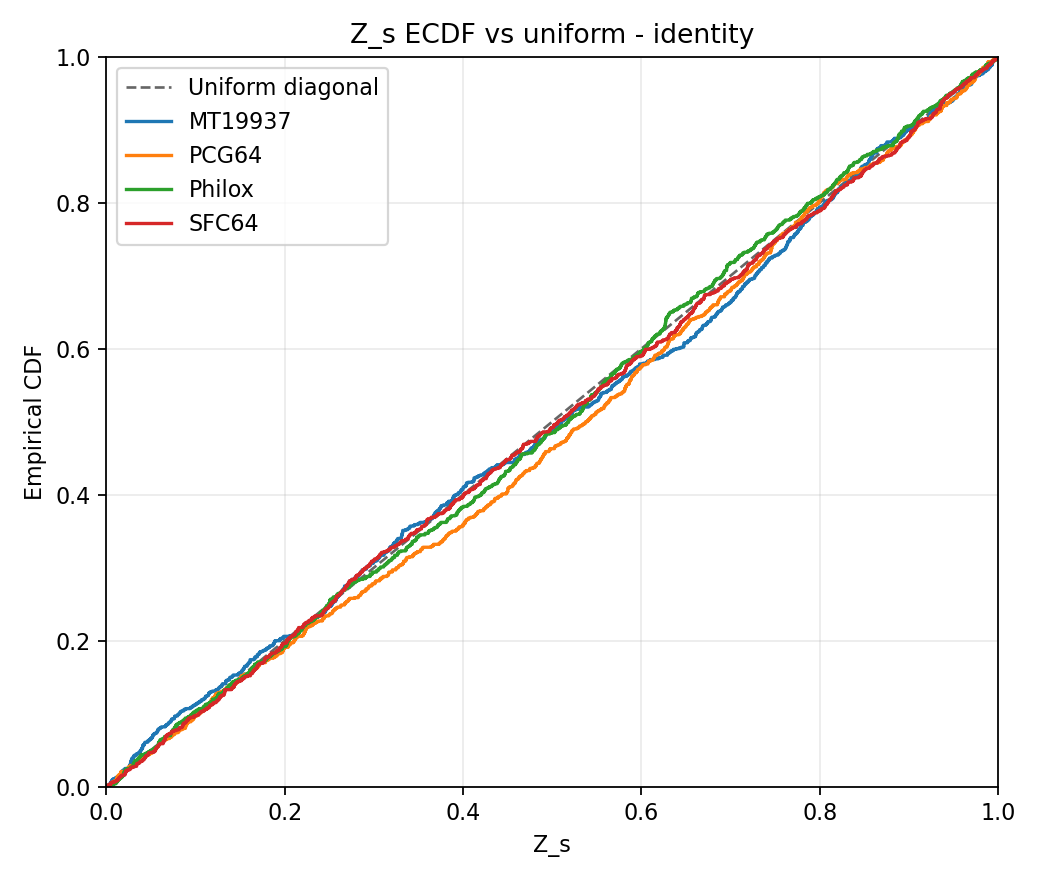
\includegraphics[width=0.92\textwidth]{figures/ecdf_Zs_identity.png}
\caption{ECDF of $Z_s$ for the identity integrand.}
\end{figure}

\begin{figure}[h]
\centering
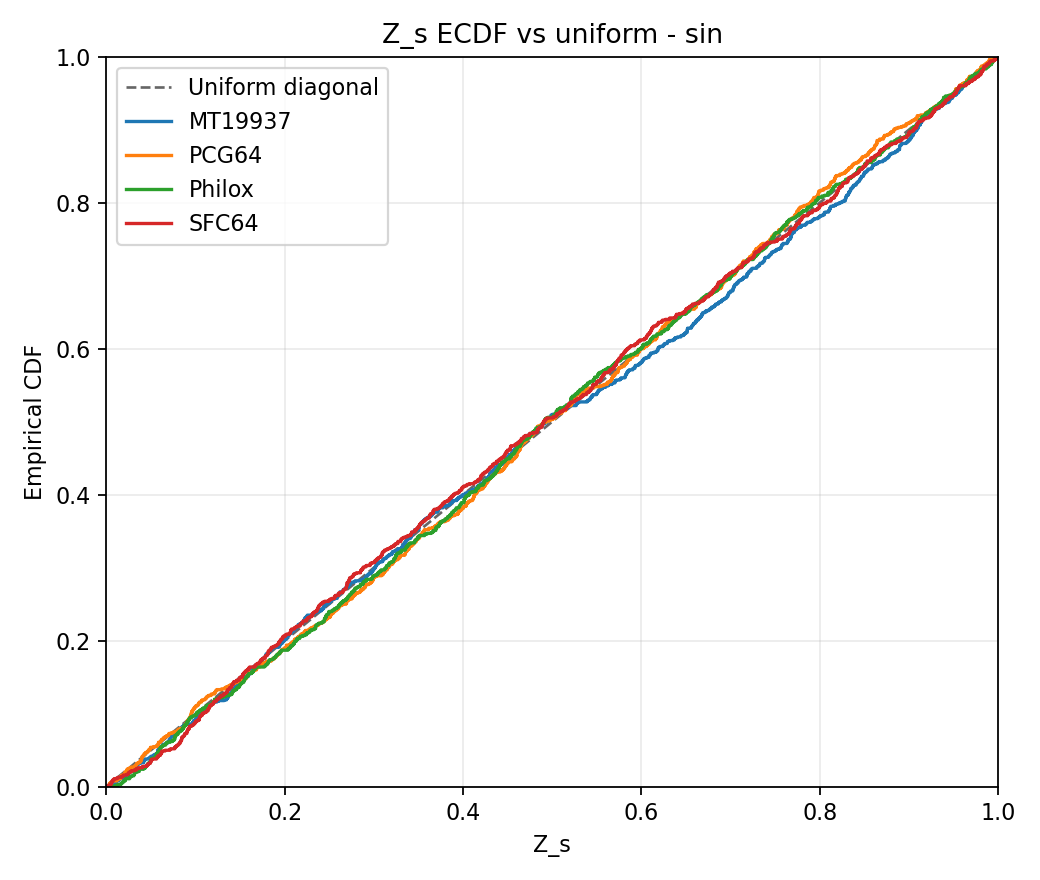
\includegraphics[width=0.92\textwidth]{figures/ecdf_Zs_sin.png}
\caption{ECDF of $Z_s$ for the sine integrand.}
\end{figure}

\begin{figure}[h]
\centering
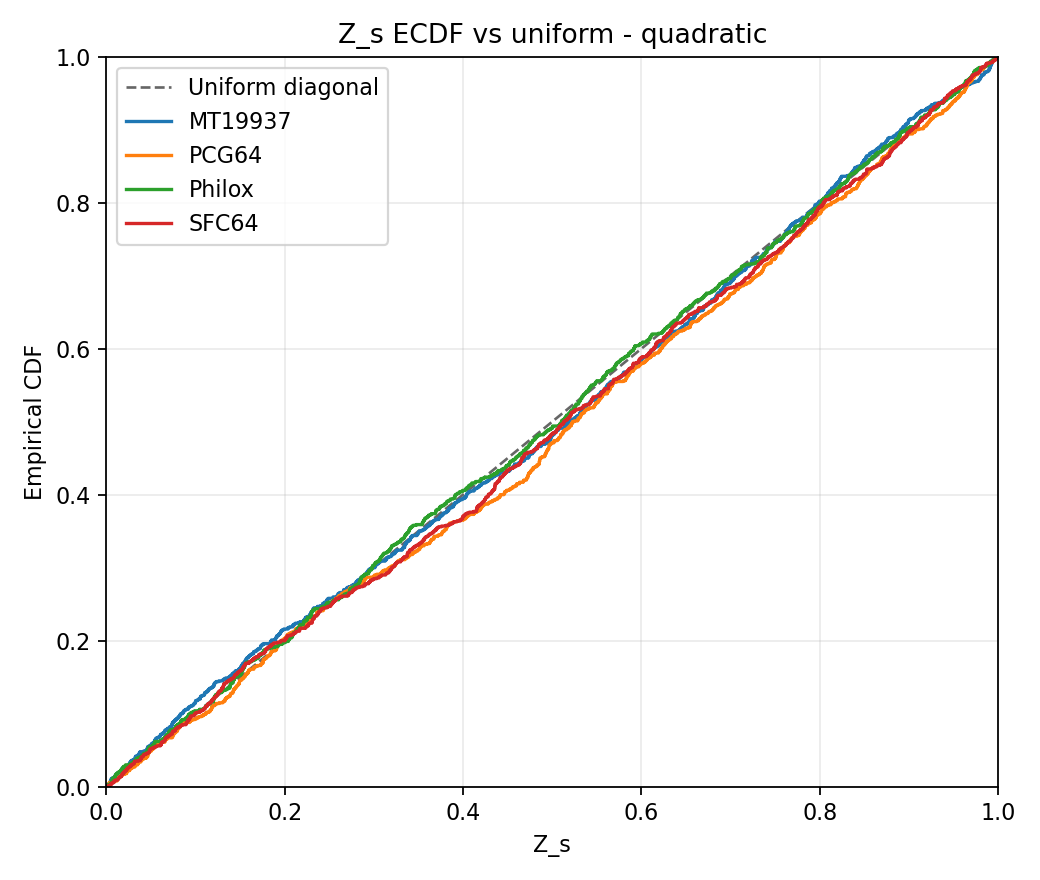
\includegraphics[width=0.92\textwidth]{figures/ecdf_Zs_quadratic.png}
\caption{ECDF of $Z_s$ for the quadratic integrand.}
\end{figure}

\begin{figure}[h]
\centering
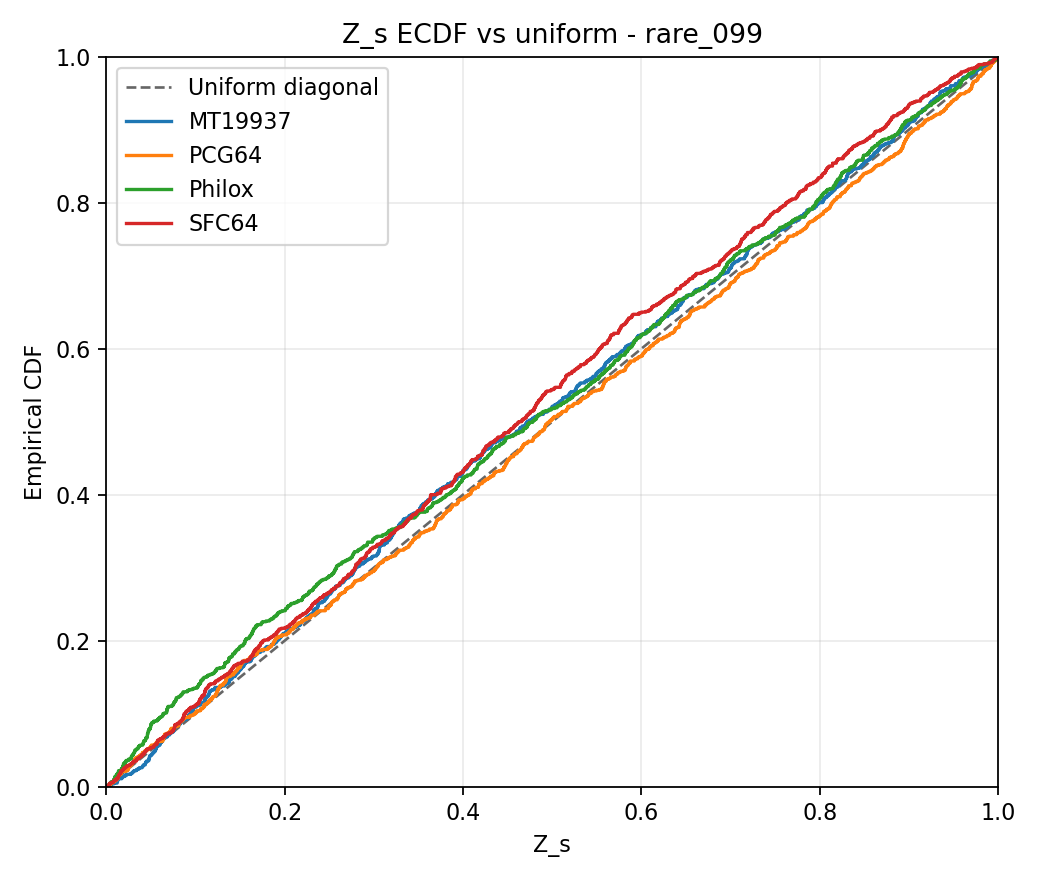
\includegraphics[width=0.92\textwidth]{figures/ecdf_Zs_rare_099.png}
\caption{ECDF of $Z_s$ for the rare-event integrand $1_{\{u>0.99\}}$.}
\end{figure}

\begin{figure}[h]
\centering
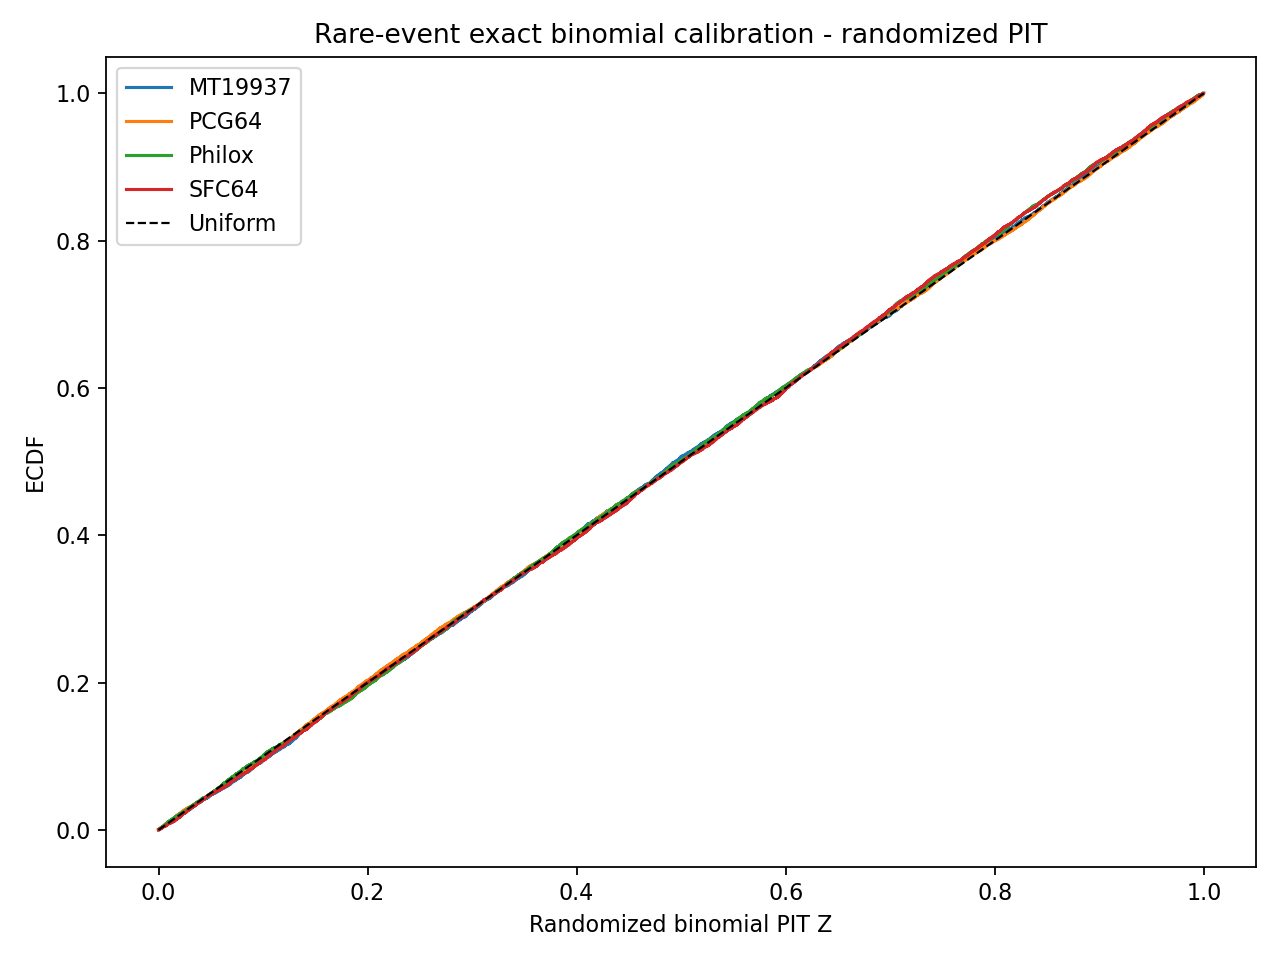
\includegraphics[width=0.92\textwidth]{figures/ecdf_Zbin_rare_099.png}
\caption{ECDF of randomized exact binomial PIT values for rare-event counts.}
\end{figure}

\clearpage
\subsection{Histograms}

\begin{figure}[h]
\centering
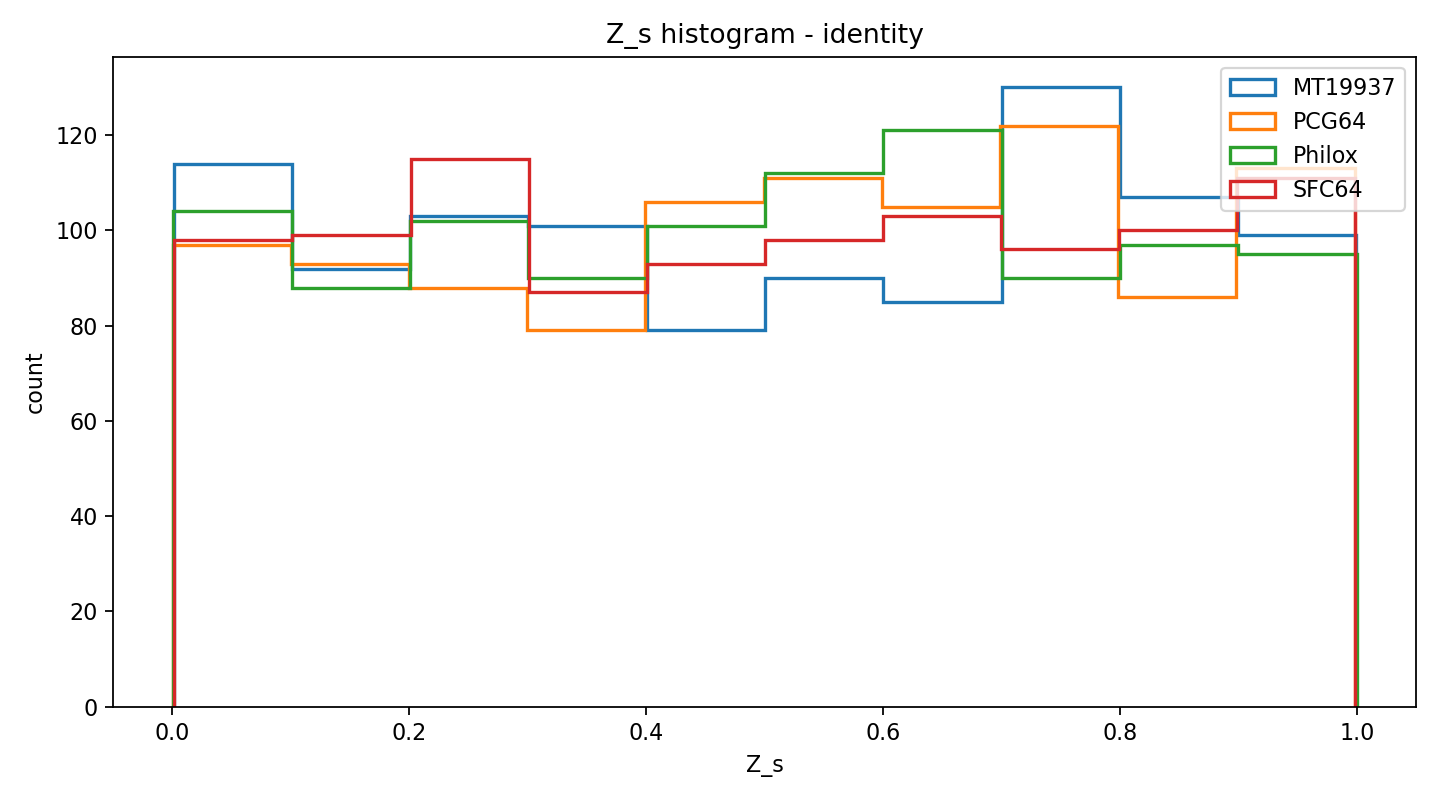
\includegraphics[width=0.92\textwidth]{figures/hist_Zs_identity.png}
\caption{Histogram of $Z_s$ for the identity integrand.}
\end{figure}

\begin{figure}[h]
\centering
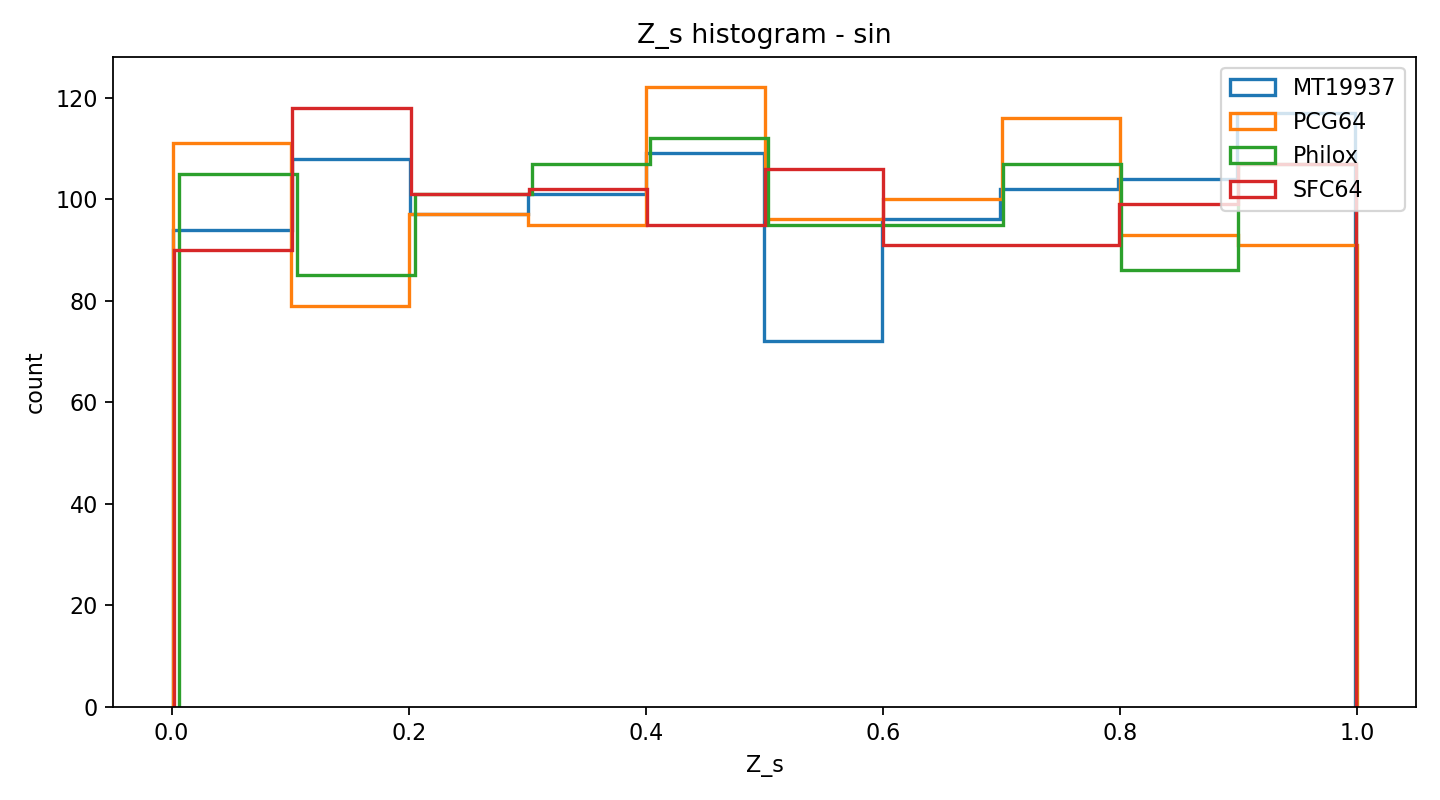
\includegraphics[width=0.92\textwidth]{figures/hist_Zs_sin.png}
\caption{Histogram of $Z_s$ for the sine integrand.}
\end{figure}

\begin{figure}[h]
\centering
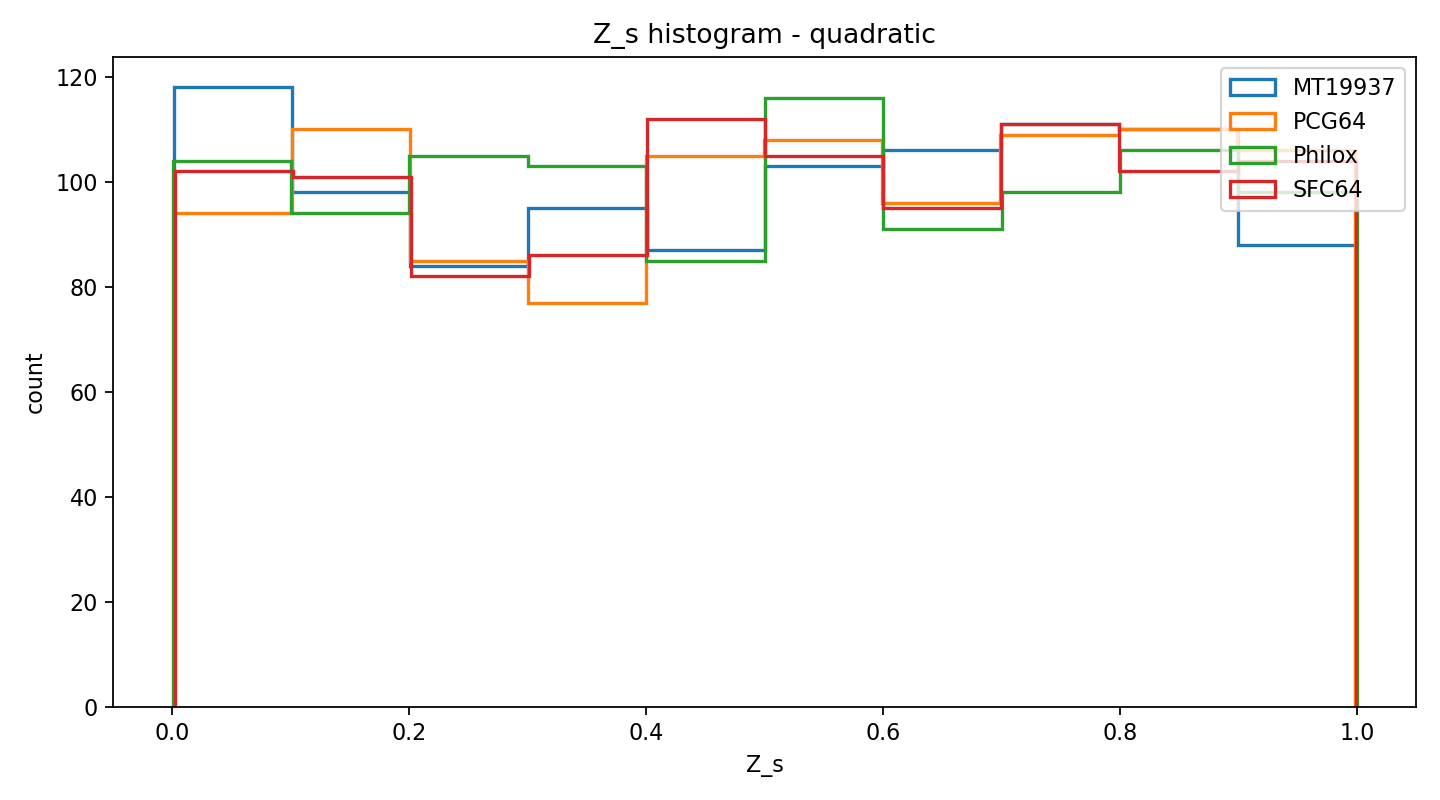
\includegraphics[width=0.92\textwidth]{figures/hist_Zs_quadratic.png}
\caption{Histogram of $Z_s$ for the quadratic integrand.}
\end{figure}

\begin{figure}[h]
\centering
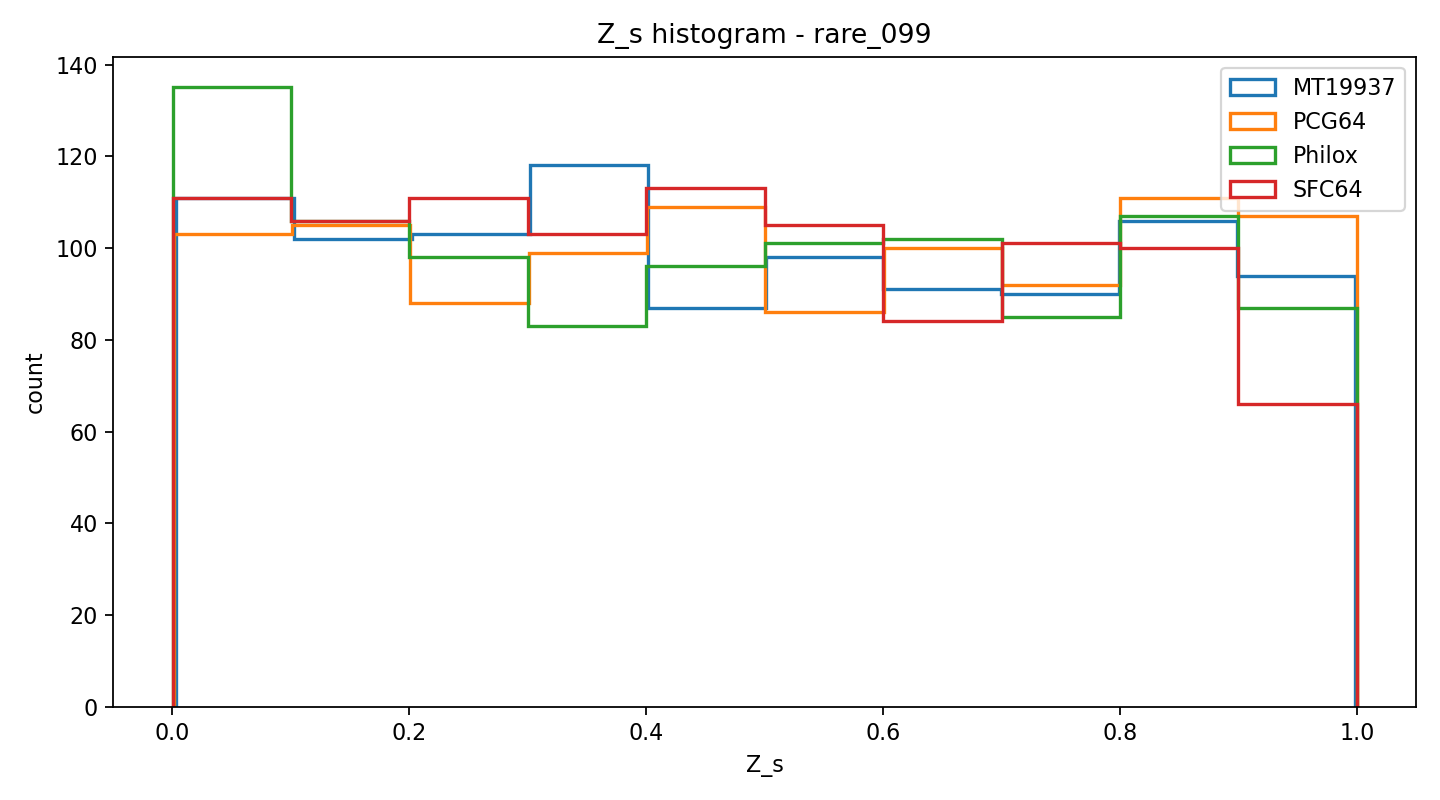
\includegraphics[width=0.92\textwidth]{figures/hist_Zs_rare_099.png}
\caption{Histogram of $Z_s$ for the rare-event integrand $1_{\{u>0.99\}}$.}
\end{figure}

\clearpage
\section{Reproducibility Manifest}

\subsection{Public baseline bundle}

\begin{verbatim}
prng-ztest/
  README.md
  requirements.txt
  scripts/
    generate_public_prng_estimates.py
    compute_z_scores.py
    plot_z_histograms.py
    plot_z_ecdf.py
  data/
    public_prng_estimates.csv
  results/
    z_scores_table.csv
    z_summary.csv
    binomial_rare_event_table.csv
    binomial_rare_event_summary.csv
  figures/
    ecdf_Zs_*.svg
    hist_Zs_*.svg
    ecdf_Zbin_rare_099.svg
    optional PNG renderings for PDF inclusion
\end{verbatim}

The scripts, requirements file, summary table and SVG figures form the recommended
versioned reproducibility bundle. The large CSV files
\texttt{data/public\_prng\_estimates.csv} and
\texttt{results/z\_scores\_table.csv} are generated locally by the commands below;
they may be archived as release artefacts rather than committed directly.

Baseline commands:
\begin{verbatim}
python scripts/generate_public_prng_estimates.py --N 50000 --R 8 --seeds 1000

python scripts/compute_z_scores.py \
  --input data/public_prng_estimates.csv \
  --out-table results/z_scores_table.csv \
  --out-summary results/z_summary.csv

python scripts/plot_z_ecdf.py \
  --input results/z_scores_table.csv \
  --outdir figures

python scripts/plot_z_histograms.py \
  --input results/z_scores_table.csv \
  --outdir figures
\end{verbatim}

\subsection{Independent-verification requirements for reported CTACM results}

For the reported Montmory\_CTACM evidence to be treated as independently reproducible, the archival bundle must include:
\begin{itemize}
  \item full SmallCrush, Crush and BigCrush logs;
  \item TestU01 version;
  \item stream adapter source or hash;
  \item backend implementation hashes;
  \item compiler flags and hardware details;
  \item seed and output horizon;
  \item SHA-256 of raw logs;
  \item CPU/Metal/CUDA stream hashes for the cross-backend replay claim.
\end{itemize}

\section{Limitations}

The present manuscript remains limited in the following ways:
\begin{itemize}
  \item $Z_s(f)$ depends on the selected null model;
  \item the $\chi^2$ calibration assumes approximately Gaussian replicated estimates;
  \item public CPU baseline integrands are simple diagnostics, not a full industrial payoff suite;
  \item no GPU public baseline is claimed in the reproducible v1.3 evidence;
  \item reported Montmory\_CTACM results require archival raw logs and stream hashes before they can be treated as independently reproducible;
  \item statistical evidence does not imply cryptographic security;
  \item passing this protocol does not prove absence of defects outside the tested seed set, workload family or horizon.
\end{itemize}

\section{Conclusion}

The consolidated result is:
\[
\boxed{
\text{Raw inter-seed variance ratios can overstate seed instability.}
}
\]
After null calibration, the verified public CPU baseline shows:
\[
\boxed{
\text{mild calibration drift in some pairs, but no strong tail pathology.}
}
\]
The exact binomial rare-event PIT check is compatible for all four tested public generators.

The scientific contribution is therefore methodological:
\[
\boxed{
\text{TACM separates raw alerts from calibrated evidence.}
}
\]
It distinguishes compatible behaviour, calibration drift and genuine tail anomaly, while preserving the non-claims required for responsible PRNG reporting.

\section{Future Work}

The next experimental additions should be:
\begin{itemize}
  \item import raw TestU01 logs and stream adapter hashes;
  \item run controlled injected marginal-bias tests;
  \item run controlled temporal-correlation tests;
  \item run rare-event deletion power tests;
  \item add backend reproducibility manifests for public generators where applicable;
  \item add multi-$S,N,R$ stability grids;
  \item extend diagnostic integrands toward finance / insurance / HPC workloads.
\end{itemize}

\begin{thebibliography}{9}
\bibitem{lecuyer2007}
P. L'Ecuyer and R. Simard, ``TestU01: A C library for empirical testing of random number generators,'' ACM Transactions on Mathematical Software, 33(4), 2007.

\bibitem{practrand}
C. Doty-Humphrey, ``PractRand statistical test suite,'' public software documentation and source distribution.

\bibitem{numpy}
C. R. Harris et al., ``Array programming with NumPy,'' Nature, 585, 357--362, 2020.

\bibitem{matsumoto1998}
M. Matsumoto and T. Nishimura, ``Mersenne Twister: A 623-dimensionally equidistributed uniform pseudo-random number generator,'' ACM TOMACS, 1998.

\bibitem{pcg}
M. E. O'Neill, ``PCG: A family of simple fast space-efficient statistically good algorithms for random number generation,'' technical report, 2014.

\bibitem{philox}
J. K. Salmon, M. A. Moraes, R. O. Dror and D. E. Shaw, ``Parallel random numbers: As easy as 1, 2, 3,'' SC11, 2011.

\bibitem{lecuyer1999}
P. L'Ecuyer, ``Good parameter sets for combined multiple recursive random number generators,'' Operations Research, 47(1), 1999.
\end{thebibliography}

\end{document}
